\subsection{Analog to Digital Converters} \label{subsec:ADCs}
The analog front-end module uses LTC2311\cite{ADC_LTC2311} 16-bit ADCs to sample the DUT voltage and current. The circuits surrounding the two ADCs are identical, so only one of them will be described here. There are several ways to drive the inputs of the ADC, as described in the datasheet \cite{ADC_LTC2311}. 
The ADC input and can be configured to sample either single-ended signals, i.e. between the signal source and a ground reference, or differential signals between two nodes as shown on the application circuit on figure \refq{fig_7_1_DRIVEADC}.

\begin{figure}[H]
    \centering
    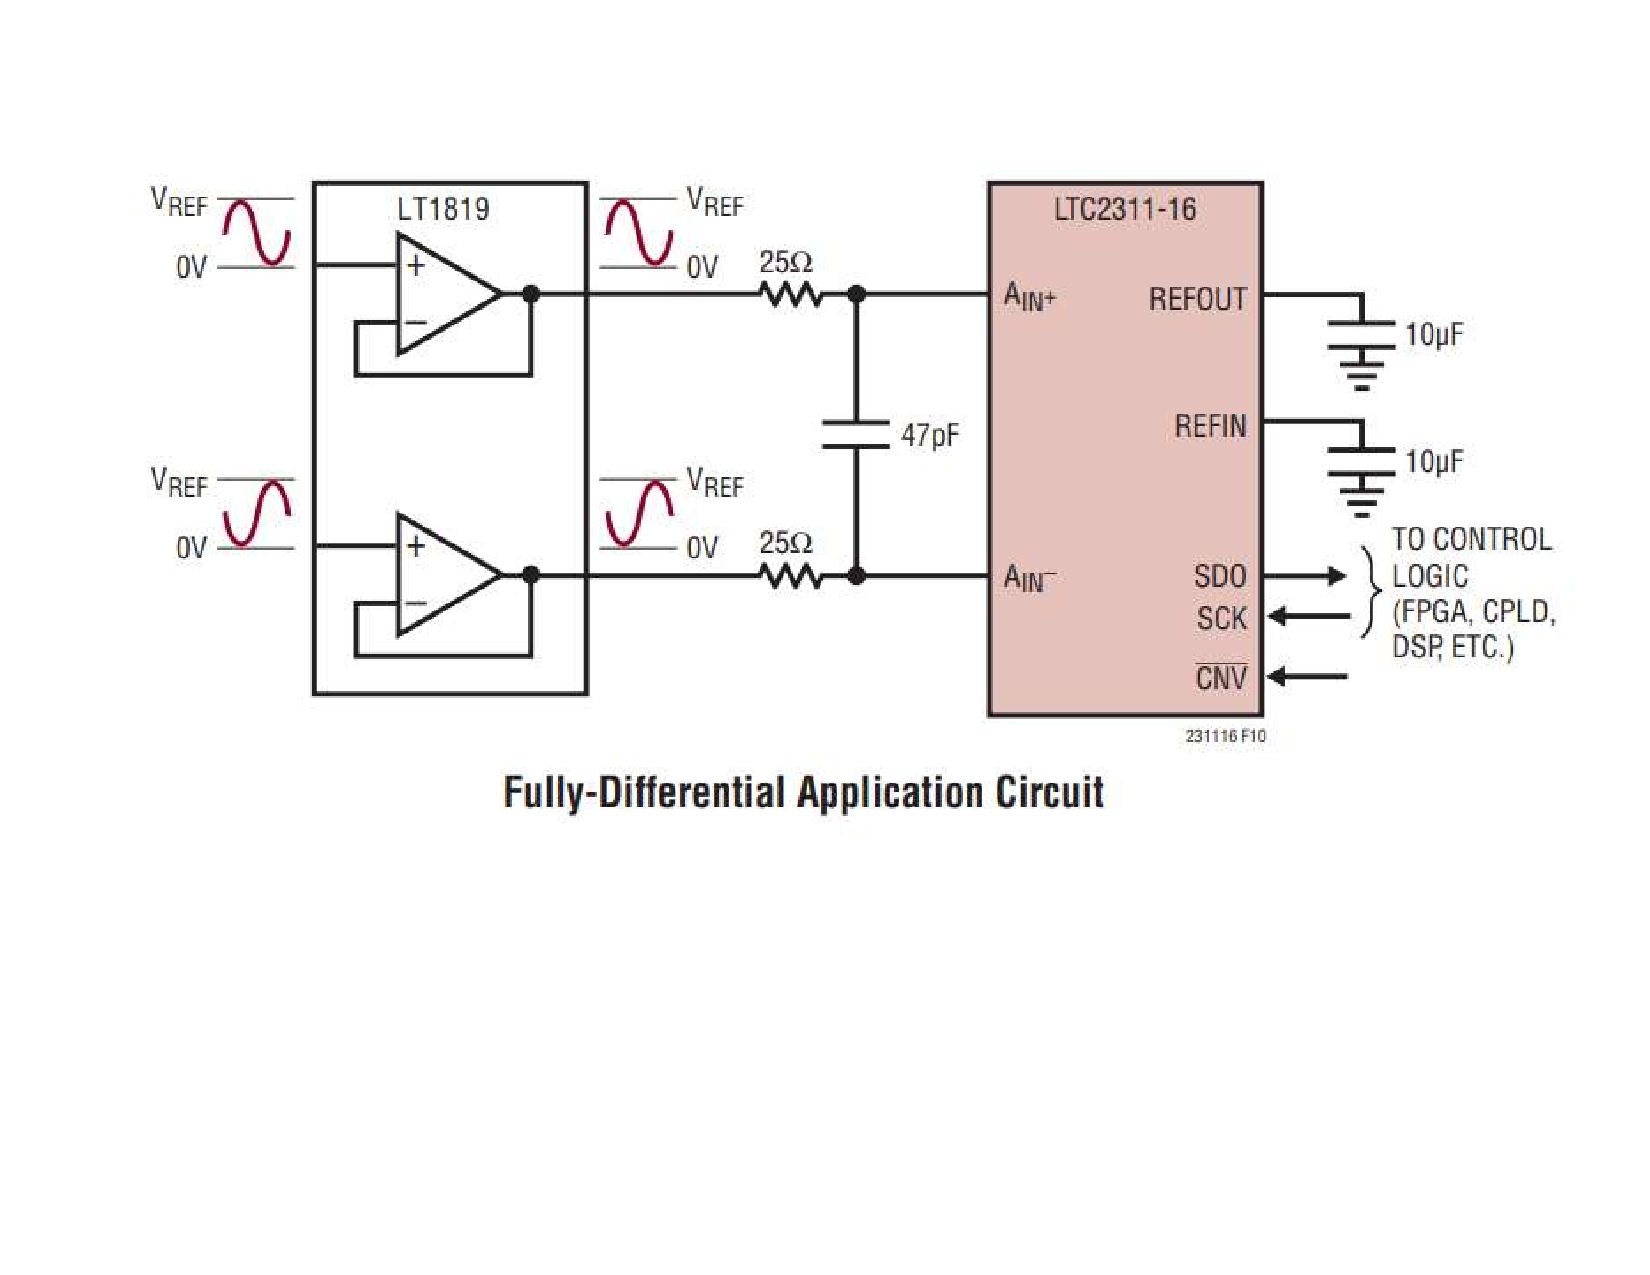
\includegraphics[clip, trim=0 200 0 50, width=1\textwidth]{Sections/7_SystemDesign/Figures/7_1_ADC_FULLDIFFINPUT.pdf}
    \caption{A schematic showing how the inputs, $A_{IN+}$ and $A_{IN-}$, of the LTC2311 ADC should be driven \cite{ADC_LTC2311} for differential signals.}
    \label{fig_7_1_DRIVEADC}
\end{figure}

Driving the ADC inputs as shown on figure \refq{fig_7_1_DRIVEADC} will give the ADC a resolution of $n = 16$ bits. Assuming an ADC reference voltage of $V_{REF} = 5 V$ the ADC will have a resolution of $V_{res} \approx 76.3 \mu V$ as shown in equation \refq{eq:7_1_2_ADCRES}. 
\begin{equation}\label{eq:7_1_2_ADCRES}
    V_{res} = \frac{V_{REF}}{2^n} = \frac{5}{2^{16}} = 7.6294e-5
\end{equation}
The application circuit shown on figure \refq{fig_7_1_DRIVEADC} is recommended for optimum performance in the datasheet and has been directly applied as-is in this project. The passive components between the LTC1819 OP-Amps and LTC2311 ADC in the application circuit is a low pass filter for filtering the noise generated by the LTC1819 buffer, it is not to be confused with an anti-aliasing filter that will be shown later in this section.

The ADC has a built-in \SIQ{4.096}{\volt} reference, but this reference is being overdriven on the 'REFOUT' pin with an external 5V reference as shown on figure \refq{fig_7_1_2_ADC5VREF}.

\begin{figure}[H]
    \centering
    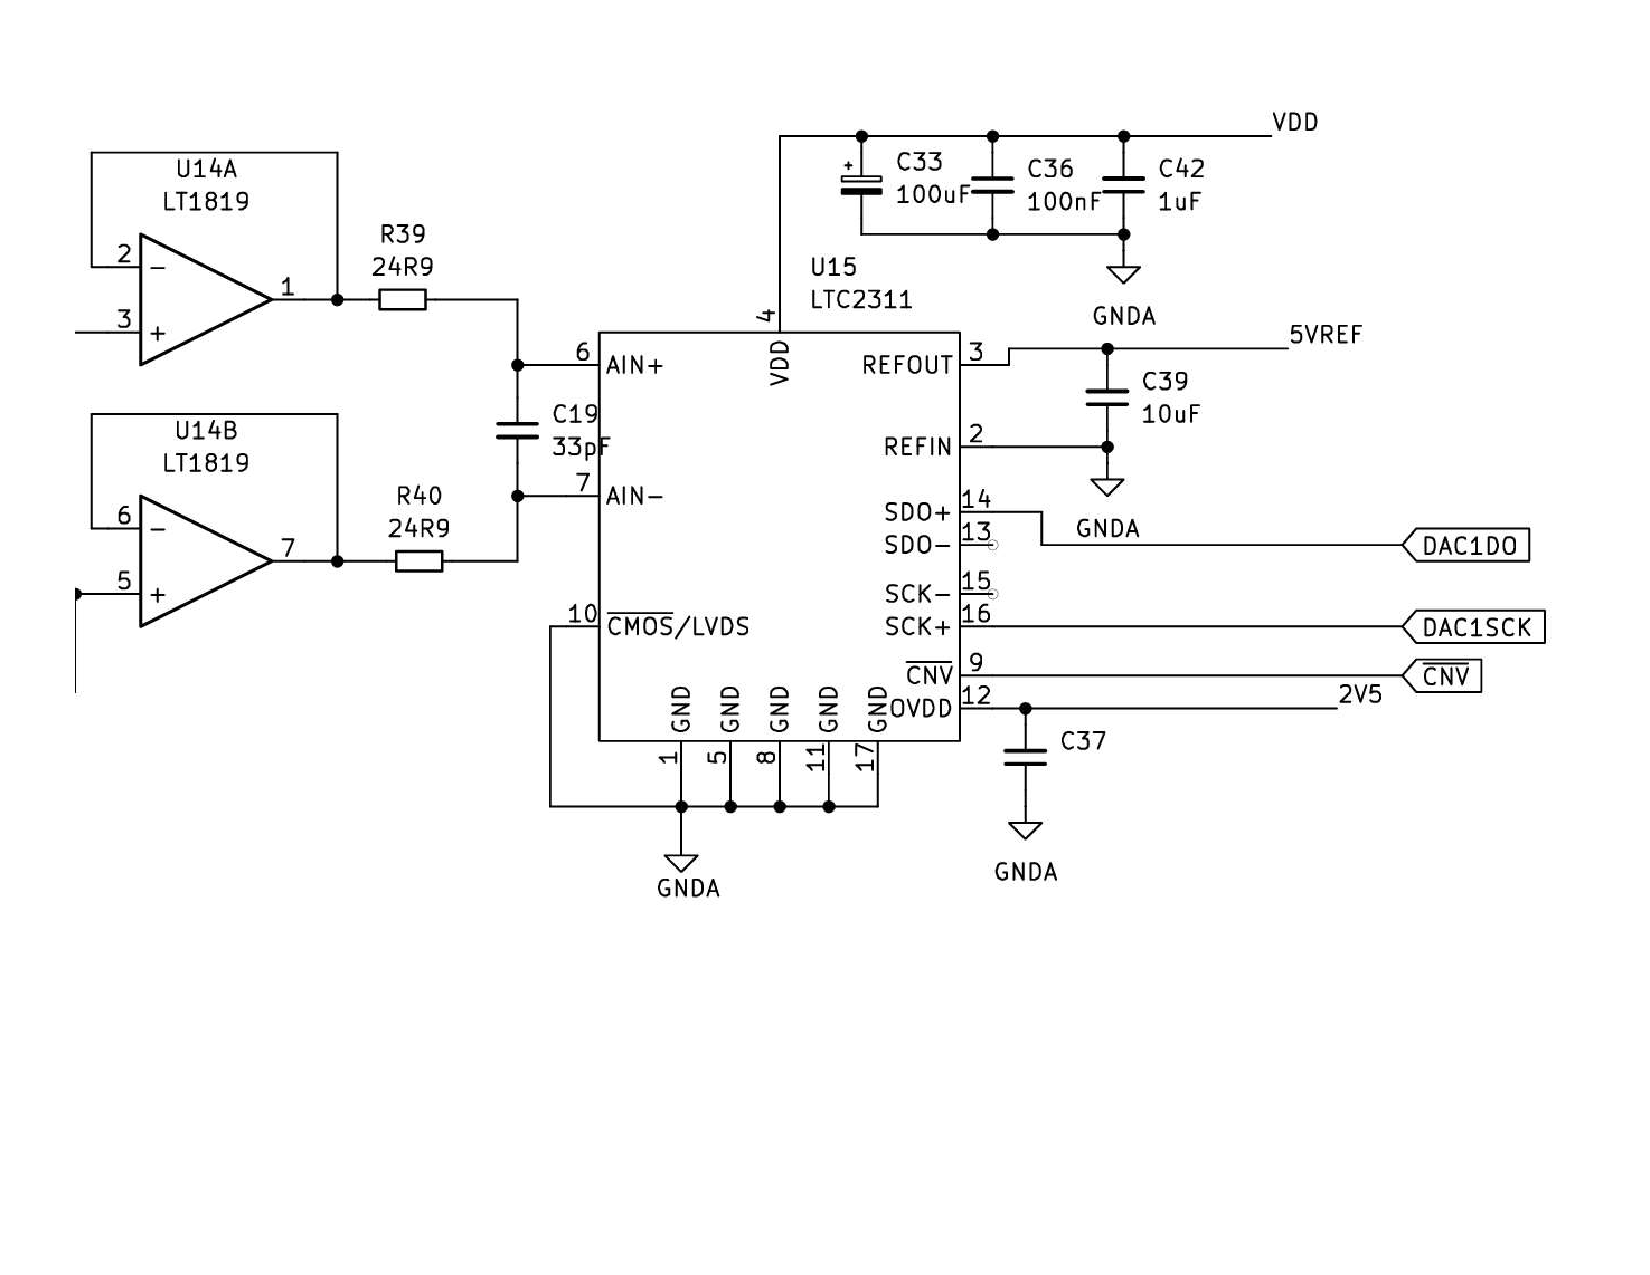
\includegraphics[clip, trim=0 150 0 0, width=1\textwidth]{Sections/7_SystemDesign/Figures/7_1_2_ADC5V.pdf}
    \caption{The REFOUT pin is overdriven on the LTC2311 to give it a 5V reference voltage.}
    \label{fig_7_1_2_ADC5VREF}
\end{figure}

Note how on the figure that the reference pins are labeled "REFIN" and "REFOUT" and that the 5V input is applied at the REFOUT pin. This is not a mistake, even if it may be counter-intuitive. When overdriving the internal reference the LTC2311s REFOUT pin must be connected to the external reference and the REFIN pin must be grounded as shown on figure \refq{fig_7_1_2_ADC5VREF}. Increasing the reference voltage from \SIQ{4.096}{\volt} to \SIQ{5}{\volt} will increase the Signal-To-Noise Ratio (SNR) of the system as larger signals can be present at the ADC inputs and make better use of the ADCs dynamic range. The pins labeled SDO, SCK, CNV is the digital interface for the LTC2311. This will be covered in detail in the documentation for the Sample Control module.

The input signals for the LTC2311 ADC may not exceed the supply voltage, which is \SIQ{5}{\volt}. To ensure this doesn't happen due to a transient event the LT1819 ADC input buffers supply will be selected to ensure this cannot happen. The typical maximum/minimum output swing from the LTC1819 is $V_{O} = \pm 4.1$V \cite{OPAMP_LT1819}. The LT1819's will have a \SIQ{+6}{\volt} and \SIQ{-1}{\volt} DC supply to both protect the ADC and to ensure that it can output the largest possible signal without clipping.  

